\documentclass{article}
%\usepackage{times}
\usepackage{graphicx}
\usepackage{grffile}
\usepackage{verbatim}
\usepackage{amsmath}
\usepackage{amssymb}
\usepackage{color}
\usepackage{float}
\usepackage{pdflscape} % landscape for pdflatex
\usepackage{wrapfig} % wrap text around figures
\usepackage{rotating}
\usepackage{mycommands}
\usepackage{afterpage}
\usepackage[top=2cm,bottom=2cm,left=2cm,right=2cm]{geometry}
\usepackage{comment} % For debugging
\usepackage{subfigure}
\usepackage{sectsty} % Set section styling
\usepackage[percent]{overpic} % For writing on top of figures
%\usepackage{hyperref} % Hyperlinks in TOC

\setlength{\abovecaptionskip}{0pt} % Space above Captions
\setlength{\belowcaptionskip}{0pt} % Space below Captions
\setlength{\floatsep}{0pt} % Space between floats
\setlength{\textfloatsep}{0pt} % Space between floats and text

%==================================
%  Define Colors
\definecolor{violet}{RGB}{238,130,238}
\definecolor{dviolet}{RGB}{148,0,211}
%==================================

% Blue Star:
\newcommand{\bstar}{{\color{blue}$\boldsymbol{\ast}$}}


% sectsty commands:
\chapterfont{\color{blue}}  % sets colour of chapters
\sectionfont{\color{dviolet}}  % sets colour of sections
\subsectionfont{\color{blue}}
\subsubsectionfont{\color{blue}}


%==============Define Symbols==============#

\def\nb {\mbox{\boldmath $\overline{\nu}$}}

\def\nm {\mbox{\boldmath $\nu_\mu$}} 
\def\anm{\mbox{\boldmath $\bar\nu_\mu$}} 
\def\ne {\mbox{\boldmath $\nu_e$}} 
\def\ane{\mbox{\boldmath $\bar\nu_e$}} 

\def\pip{\mbox{\boldmath $\pi^+$}} 
\def\pim{\mbox{\boldmath $\pi^-$}} 
\def\mup{\mbox{\boldmath $\mu^+$}} 
\def\mum{\mbox{\boldmath $\mu^-$}} 
\def\kap{\mbox{\boldmath $K^+$}} 
\def\kam{\mbox{\boldmath $K^-$}} 
\def\kl {\mbox{\boldmath $K^0_L$}} 
\def\ks {\mbox{\boldmath $K^0_S$}} 


\def\nmne{\mbox{\boldmath $\nu_{\mu}\rightarrow\nu_{e}$}} 
\def\nmnt{\mbox{\boldmath $\nu_{\mu}\rightarrow\nu_{\tau}$}} 
\def\nmnx{\mbox{\boldmath $\nu_\mu\rightarrow\nu_x$}} 
\def\nent{\mbox{\boldmath $\nu_e\rightarrow\nu_\tau$}} 
\def\nenx{\mbox{\boldmath $\nu_e\rightarrow\nu_x$}} 

\def\enu {\mbox{\boldmath $E_{\nu}$}}
\def\emu {\mbox{\boldmath $E_{\mu}$}}
\def\eh{\mbox{\boldmath $E_{Had}$}}

\def\nova{NO$\nu$A} 
\def\cohp{\boldmath {Coh$\pi^0$} }
\def\cohpip{\boldmath {Coh$\pi^+$} }
\def\cohpiz{\boldmath {Coh$\pi^0$} }
\def\cohr{\boldmath {Coh$\rho^0$} }
\def\cohrz{\boldmath {Coh$\rho^0$} }
\def\cohrp{\boldmath {Coh$\rho^+$} }
\def\cohphi{\boldmath {Coh$\phi^0$} }
\def\cohjp{\boldmath {Coh$J/\psi$} }
\def\piz{\boldmath {$\pi^0 $} }
\def\mpiz{\boldmath {M$_\pi^0 $} }
\def\mgg{\boldmath {M$_{\gamma \gamma} $} }
\def\gam{\boldmath {$\gamma $} }
\def\gf{\boldmath {$\gamma 1$} }
\def\gs{\boldmath {$\gamma 2$} }
\def\A{\boldmath {${\cal A}$} }
\def\zt{\boldmath {$\zeta$}}
\def\ztp{\boldmath {$\zeta_{\pi^0}$}}
\def\ztgg{\boldmath {$\zeta_{\gamma \gamma}$}}
\def\ztf{\boldmath {$\zeta_{\gamma 1}$}}
\def\zts{\boldmath {$\zeta_{\gamma 2}$}}
\def\thfs{\boldmath {$\Theta_{1 2}$}}

\def\zetap{\boldmath {$\zeta_{K^{+}}$}}
\def\zetam{\boldmath {$\zeta_{K^{-}}$}}
\def\zetar{\boldmath {$\zeta_{\pi \pi}$}}
\def\zetaphi{\boldmath {$\zeta_{KK}$}}
\def\phiop{\boldmath {$\phi_{12}$}}

\def\pkpos{\boldmath {$P_{K^{+}}$}}
\def\pkneg{\boldmath {$P_{K^{-}}$}}

\def\ptr{\boldmath {$P_{t} \pi \pi$}}
\def\ptphi{\boldmath {$P_{t} KK$}}
\def\ptpipos{\boldmath {$P_{t} \pi^{+}$}}
\def\ptpineg{\boldmath {$P_{t} \pi^{-}$}}
\def\ptkpos{\boldmath {$P_{t} K^{+}$}}
\def\ptkneg{\boldmath {$P_{t} K^{-}$}}

\def\erho{\boldmath {$E_{\pi \pi}$}}
\def\ephi{\boldmath {$E_{KK}$}}
\def\pphi{\boldmath {$P_{KK}$}}
\def\thetar{\boldmath {$\theta_{\pi \pi}$}}
\def\thetaphi{\boldmath {$\theta_{KK}$}}
\def\thetaop{\boldmath {$\theta_{12}$}}
\def\thetap{\boldmath {$\theta_{K^{+}}$}}
\def\thetam{\boldmath {$\theta_{K^{-}}$}}

\def\mpipi{\boldmath {$M_{\pi \pi}$}}
\def\mkk{\boldmath {$M_{KK}$}}

\def\phipt{\boldmath {$\phi_{KK}$}}

%========================================%
% Add a figure with captions HERE!
% 1st argument: Filename
% 2nd argument: Size in ratio of \textwidth
% 3rd argument: Caption
%
% Example:
%    \addfig{foo.pdf}{0.9}{A foo caption}
\newcommand{\addfig}[3]{
\begin{figure}[h!]
\begin{center}
\includegraphics[width=#2\textwidth]{#1}
\caption{#3   \textbf{(#1)}}
\end{center}
\end{figure}
}
%========================================%
% Two figures side-by-side
% 1st argument: First Filename
% 2nd argument: First Caption
% 3rd argument: Second Filename
% 4th argument: Second Caption
% 5th argument: Total Caption
% 6th argument: Size of each in ratio of \textwidth (should be near 0.45)
\newcommand{\twofig}[6]{
\begin{figure}[ht]
\centering
\subfigure[#2 \textbf{(#1)}]{
	\includegraphics[width=#6\textwidth]{#1}}
\quad
\subfigure[#4 \textbf{(#3)}]{
	\includegraphics[width=#6\textwidth]{#3}}
\caption{#5}
\end{figure}
}
%========================================%
% Two figures side-by-side in landscape
% 1st argument: First Filename
% 2nd argument: First Caption
% 3rd argument: Second Filename
% 4th argument: Second Caption
% 5th argument: Total Caption
% 6th argument: Size of each in ratio of \textwidth (should be near 0.45)
\newcommand{\twofigls}[6]{
\clearpage\newpage
\begin{landscape}
\begin{figure}[ht]
\centering
\subfigure[#2 \textbf{(#1)}]{
	\includegraphics[width=#6\textwidth]{#1}}
\quad
\subfigure[#4 \textbf{(#3)}]{
	\includegraphics[width=#6\textwidth]{#3}}
\caption{#5}
\end{figure}
\end{landscape}
}
%========================================%
% Two figures up-down
% 1st argument: First Filename
% 2nd argument: First Caption
% 3rd argument: Second Filename
% 4th argument: Second Caption
% 5th argument: Total Caption
\newcommand{\twofigud}[5]{
\begin{figure}[ht]
\centering
\subfigure[#2 \textbf{(#1)}]{
	\includegraphics[width=0.5\textwidth]{#1}}
\quad
\subfigure[#4 \textbf{(#3)}]{
	\includegraphics[width=0.5\textwidth]{#3}}
\caption{#5}
\end{figure}
}
%========================================%
% Three figures grouped
% 1st argument: First Filename
% 2nd argument: First Caption
% 3rd argument: Second Filename
% 4th argument: Second Caption
% 5th argument: Third Filename
% 6th argument: Third Caption
% 7th argument: Total Caption
\newcommand{\threefig}[7]{
\begin{figure}[h!]
\centering
\subfigure[#2 \textbf{(#1)}]{
	\includegraphics[width=0.45\textwidth]{#1}}
\quad
\subfigure[#4 \textbf{(#3)}]{
	\includegraphics[width=0.45\textwidth]{#3}}
\subfigure[#6 \textbf{(#5)}]{
	\includegraphics[width=0.45\textwidth]{#5}}
\caption{#7}
\end{figure}
}
%========================================%
% Four figures grouped
% 1st argument: First Filename
% 2nd argument: First Caption
% 3rd argument: Second Filename
% 4th argument: Second Caption
% 5th argument: Third Filename
% 6th argument: Third Caption
% 7th argument: Fourth Filename
% 8th argument: Fourth Caption
% 9th argument: Total Caption
\newcommand{\fourfig}[9]{
\begin{figure}[ht]
\centering
\subfigure[#2 \textbf{(#1)}]{
	\includegraphics[width=0.45\textwidth]{#1}}
\quad
\subfigure[#4 \textbf{(#3)}]{
	\includegraphics[width=0.45\textwidth]{#3}}
\subfigure[#6 \textbf{(#5)}]{
	\includegraphics[width=0.45\textwidth]{#5}}
\quad
\subfigure[#8 \textbf{(#7)}]{
	\includegraphics[width=0.45\textwidth]{#7}}
\caption{#9}
\end{figure}
}
%========================================%
%========================================%
% Overpic Placement
% 1st argument: First filename
% 2nd argument: Second filename
% 3rd argument: X-Position
% 4rd argument: Y-Position
\newcommand{\opic}[4]{
\clearpage\newpage
%\begin{overpic}[width=1.0\textwidth,grid,tics=10] %Print grid for positioning
\begin{overpic}[width=1.0\textwidth]
{#1}
\put(#3,#4){\includegraphics[width=0.65\textwidth]{#2}}
\end{overpic}
}
%========================================%
%========================================%





\begin{document}


\title{CohJ/$\psi$ Analysis ($\boldsymbol{\nu_\mu}$ \textbf{CC})(\textbf{Coil})(\textbf{2-track})}
\author{Chris Kullenberg}
\date{\today}

\maketitle

\vspace{\fill}



%=========================================================================>
%=========================================================================>
%=========================================================================>

%0o0o0o0o0o0o0o0o0o0o0o0o0o0o0o0o0o0o0o0o0o0o0o0o0o0o0o0o0o0o0o0o0o0
%0o0o0o0o0o0o0o0o0o0o0o0o0o0o0o0o0o0o0o0o0o0o0o0o0o0o0o0o0o0o0o0o0o0
% Zeroth Norms
\clearpage\newpage

\section{Zeroth Norms}
\label{sec-zeroth-norms}

%  Table \ref{tab-gen-numbers} shows the generated,
%  MC-Z-weighted number of events to pass basic
%  cuts.  These numbers are used for weighting to the
%  desired number of "Zeroth Norm" events.

%\vspace{3ex}
%  \textbf{The cuts include:}
%  \begin{enumerate}
%    \item Fid $|$x,y-5$|$$\leq$130 ;  5$<$zvs$<$405
%    \item  Pfermi cut
%    \item $W^{2}$ cut (DIS only)
%  \end{enumerate}
%\vspace{3ex}

\vspace{5ex}

 \begin{table}[h!]\centering
 {\large{
 \begin{tabular}{||l|r|r||}
 \hline
 \hline
       & Gen Number   & Zroth Norm  \\
 \hline
           &  4116629.0 &  1440000.0 \\
 CCDIS     &  2451852.2 &   547200.0 \\
           &   337363.3 &       29.6 \\
           &   824186.4 &    10000.0 \\
 JPsi      &   147680.4 &     7380.1 \\
           &   384881.8 &    36000.0 \\
 OBG       &   418257.5 &    32000.0 \\
           &   179844.8 &     5000.0 \\
 CohPi+    &   396271.9 &    21600.0 \\
           &   193616.5 &     2160.0 \\
 CohRho+   &   189598.9 &    13680.0 \\
           &    25235.8 &     1000.0 \\
 aNuMu CC  &   934139.8 &    50400.0 \\
           &     4075.9 &      200.0 \\
 QE        &     4500.0 &      100.0 \\
           &     4500.0 &      100.0 \\
 CohPi0    &     4500.0 &      100.0 \\
           &     4500.0 &      100.0 \\
  Nue CC   &     4500.0 &      100.0 \\
           &     4500.0 &      100.0 \\
 aNue CC   &     4500.0 &      100.0 \\
           &     4500.0 &      100.0 \\
 \hline
 \hline
 \end{tabular}
 \caption{Generated Number of MC Events}
 \label{tab-gen-numbers}
 }}
 \end{table}
 \endinput


\vspace{5ex}
\begin{itemize}
\item[] \textbf{\underline{\color{dviolet} Extra Normalizations:}}
\item[\bstar] Coh$\boldsymbol{\pi^+}$: 0.985 \;\;\; (From 2V0 analysis)
\item[\bstar] Coh$\boldsymbol{\pi^0}$: 0.985 \;\;\; (From 2V0 analysis)
\item[\bstar] Coh$\boldsymbol{\rho^+}$: 0.669 \;\;\; (From CohRho0 measurment)
\item[\bstar] Coh$\boldsymbol{\rho^0}$: 0.669 \;\;\; (From CohRho0 measurment)
\item[\bstar] OBG: 0.22 (from CohRho0 analysis)
\end{itemize}


%0o0o0o0o0o0o0o0o0o0o0o0o0o0o0o0o0o0o0o0o0o0o0o0o0o0o0o0o0o0o0o0o0o0
%0o0o0o0o0o0o0o0o0o0o0o0o0o0o0o0o0o0o0o0o0o0o0o0o0o0o0o0o0o0o0o0o0o0
% Data Fit
\clearpage\newpage

% 150MeV fit:
\begin{figure}
\begin{minipage}[c]{0.76\textwidth}
    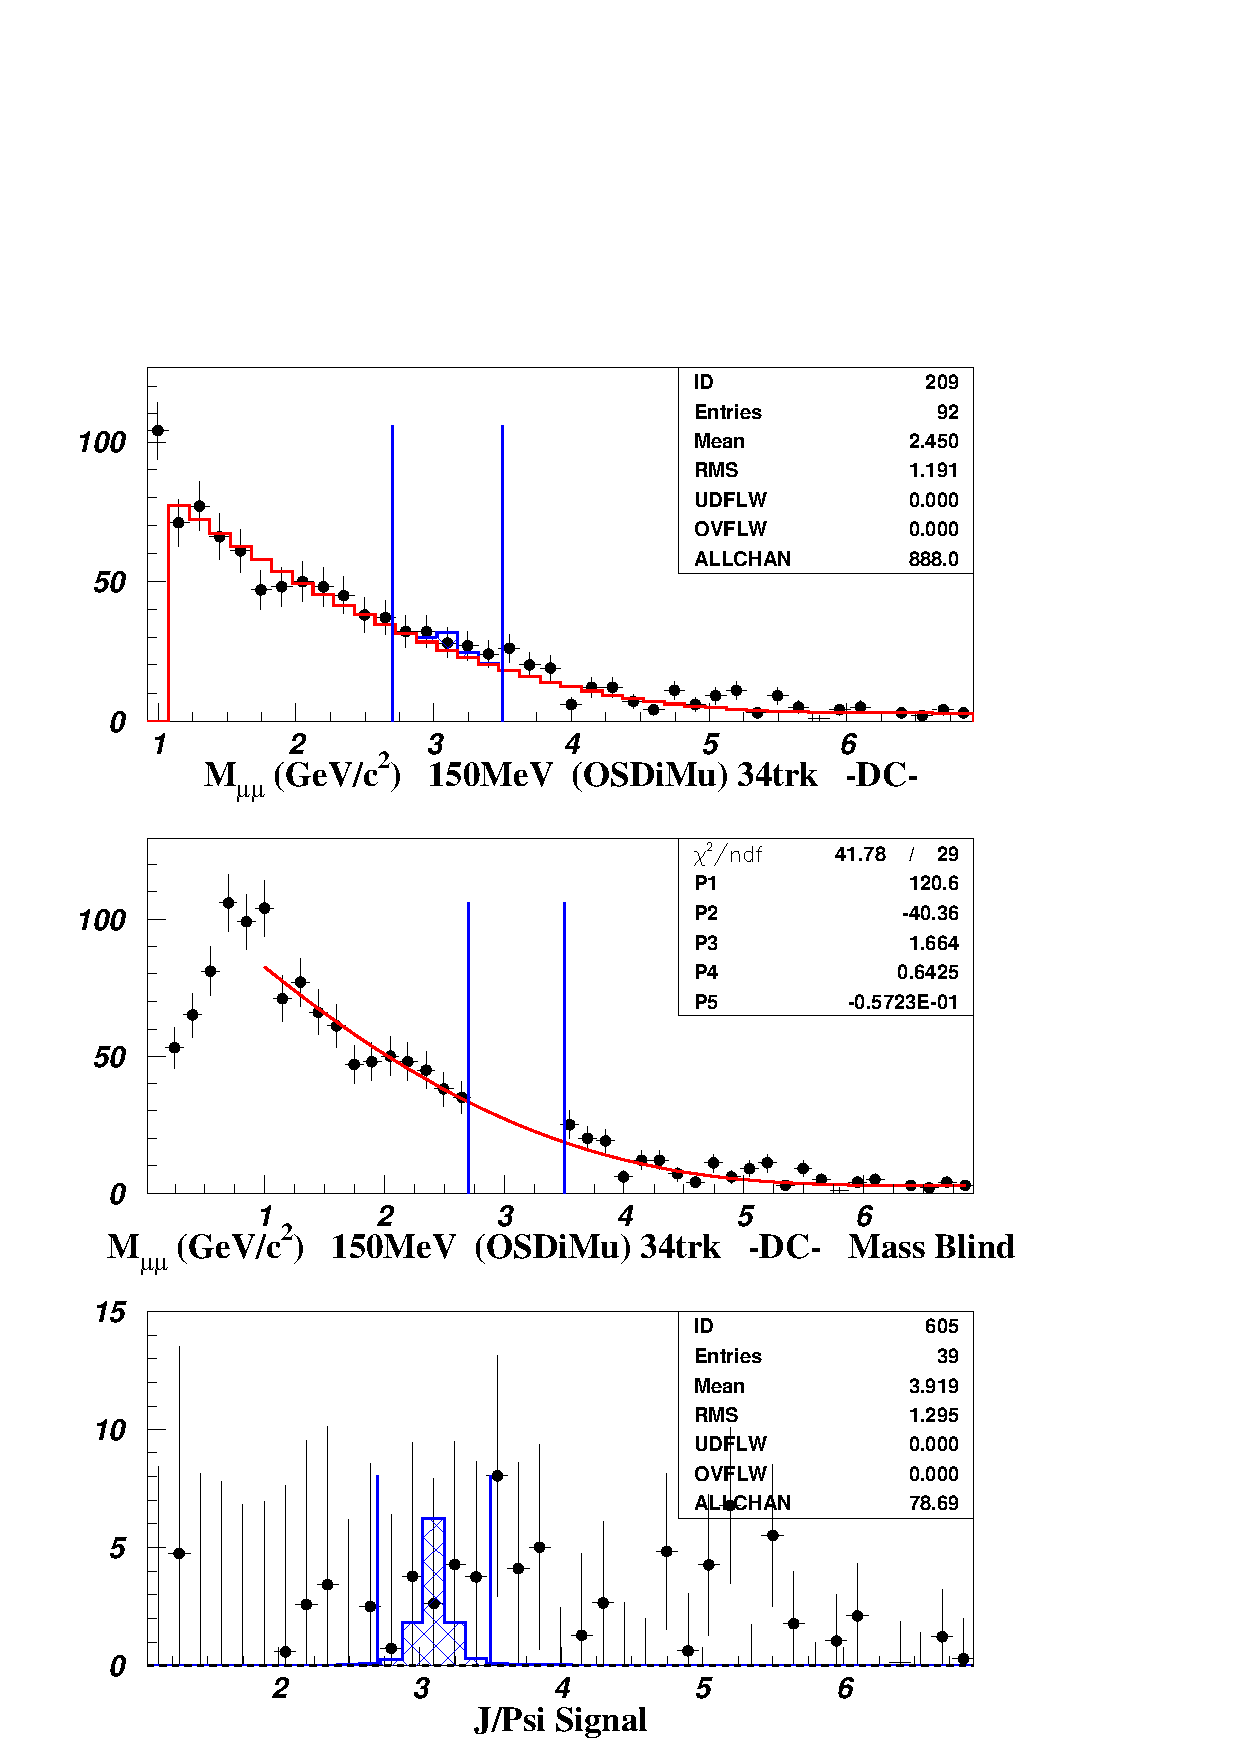
\includegraphics[width=\textwidth]{./figs/data-fit-150mev.pdf}
\end{minipage}%
\begin{minipage}[c]{0.2\textwidth}
../../../../hbook/calc_jpsi/tables/sigcalc_numucc_coil_ncand4_150mev.tex
\end{minipage}
    \caption{150MeV Data Fit. Signal MC set to calculations in 2nd range. \textbf{(./figs/data-fit-150mev.pdf)(sigcalc-150mev.tex)}}
\end{figure}

% 100MeV fit:
\begin{figure}
\begin{minipage}[c]{0.76\textwidth}
    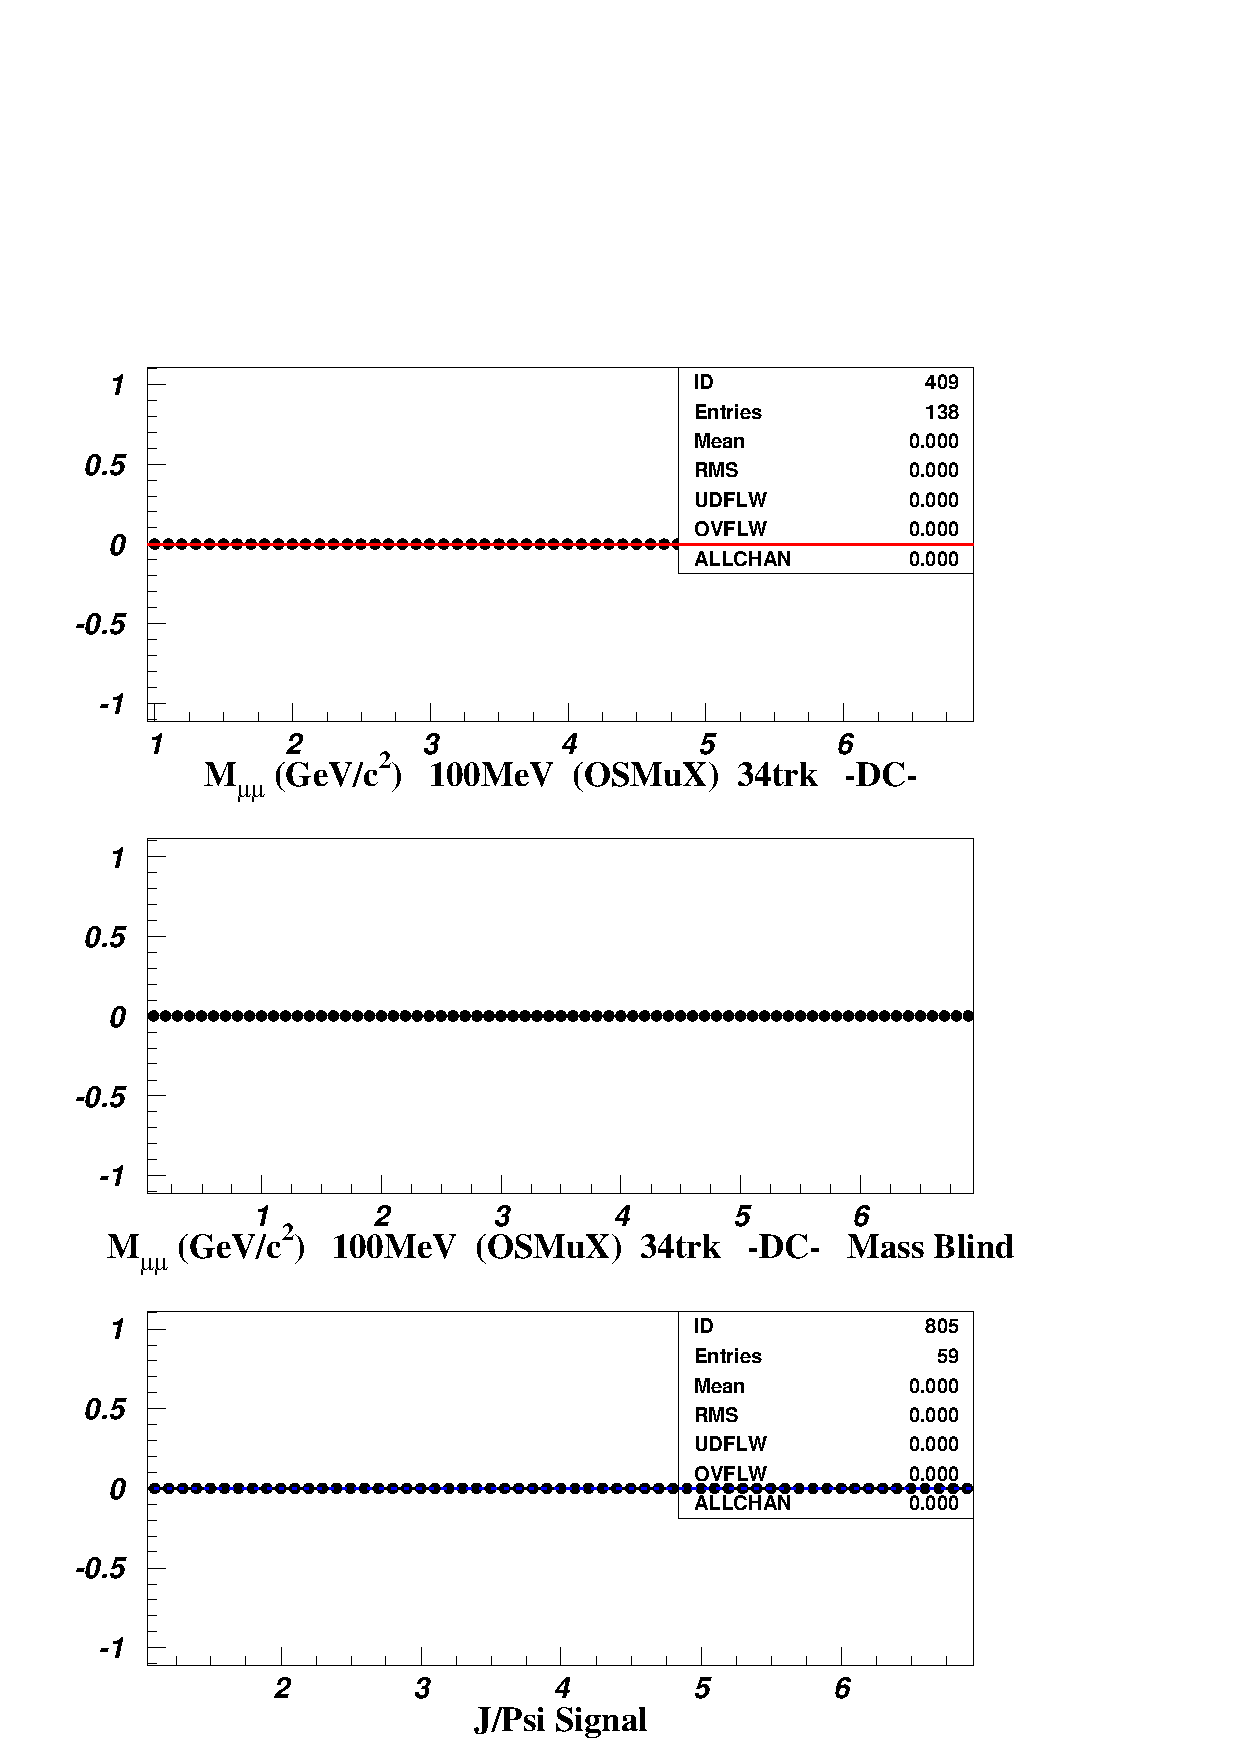
\includegraphics[width=\textwidth]{./figs/data-fit-100mev.pdf}
\end{minipage}%
\begin{minipage}[c]{0.2\textwidth}
../../../../hbook/calc_jpsi/tables/sigcalc_lsdimu_coil_ncand4_100mev.tex
\end{minipage}
    \caption{100MeV Data Fit. Signal MC set to calculations in 2nd range. \textbf{(./figs/data-fit-100mev.pdf)(sigcalc-150mev.tex)}}
\end{figure}

%0o0o0o0o0o0o0o0o0o0o0o0o0o0o0o0o0o0o0o0o0o0o0o0o0o0o0o0o0o0o0o0o0o0
%0o0o0o0o0o0o0o0o0o0o0o0o0o0o0o0o0o0o0o0o0o0o0o0o0o0o0o0o0o0o0o0o0o0
% MC Chisq Fit
\clearpage\newpage
\section{MC $\chi^2$ Fit}

\addfig{./figs/mass-0.9to5-150mev.pdf}{0.8}{}

\clearpage\newpage
\addfig{chisq-jpsi.pdf}{0.7}{}
 \begin{table}[h!]\centering
 {\small{
 \begin{tabular}{||l||r||r||}
 \hline
 \hline
\multicolumn{2}{||c||}{$\chi^{2}$ Min  41.231} & \\
 \multicolumn{2}{||c||}{Number of bins used:   29.} & \\
\multicolumn{2}{||c||}{One $\sigma$:    1.192} & \\
 \hline
 \hline
    & JPsi & \\
Norm at Min $\chi^{2}$  &   1.703 & \\
$-1$ $\sigma$ &   1.091  &  $($ 35.9$\%)$  \\
$+1$ $\sigma$ &   2.315  &  $($ 35.9$\%)$  \\
 \hline
 \hline
 \end{tabular}
 \caption{$\chi^{2}$ for JPsi on plot: 'Mmumu'}
 \label{tab-chijpsi}
 }}
 \end{table}
 \endinput

\clearpage\newpage
\addfig{chisq-cohpip.pdf}{0.7}{}
../../../../../chisq_iterative/output/mumu2/chisq_cohpip.tex
\clearpage\newpage
\addfig{chisq-ccdis.pdf}{0.7}{}
../../../../../chisq_iterative/output/mux34/chisq_ccdis.tex


%0o0o0o0o0o0o0o0o0o0o0o0o0o0o0o0o0o0o0o0o0o0o0o0o0o0o0o0o0o0o0o0o0o0
%0o0o0o0o0o0o0o0o0o0o0o0o0o0o0o0o0o0o0o0o0o0o0o0o0o0o0o0o0o0o0o0o0o0
% Summary Cut Tables 
\clearpage\newpage
\section{Summary Cut Tables}

 \begin{table}[h!]\centering
 {\small{
\begin{tabular}{||l||r|r|r|r|r||r||r||} 
 \hline
Cut Name           &  CCDIS    & \cohpip   & \cohrp    & \cohjp    & Other  &   Total   &   Data    \\ \hline  \hline
  1) Raw Events           &    1942.2 &   12354.9 &    5034.4 &      47.5 &    3968.7 &   23347.7 &   10253.0 \\
  2) OBGfid,Trig+CohGenTh &    1942.2 &   12354.9 &    5034.4 &      47.5 &    3968.7 &   23347.7 &   10253.0 \\
  3) Pfermi \& W2         &    1942.2 &   12354.9 &    5034.4 &      47.5 &    3968.7 &   23347.7 &   10253.0 \\
  4) Fid. Vol. -X         &    1828.8 &   11804.8 &    4811.1 &      45.5 &    3758.5 &   22248.6 &    9028.0 \\
  5) Fid. Vol. -Y         &    1697.0 &   11346.3 &    4616.0 &      43.8 &    3550.5 &   21253.5 &    7591.0 \\
  6) Fid. Vol. -Z (OFF)   &    1697.0 &   11346.3 &    4616.0 &      43.8 &    3550.5 &   21253.5 &    7591.0 \\
  7) At Least 1 Mu        &    1697.0 &   11196.9 &    4263.7 &      43.8 &     277.3 &   17478.7 &    7591.0 \\
  8) ncand=2,3,4          &    1697.0 &   11196.9 &    4263.7 &      43.8 &     277.3 &   17478.7 &    7591.0 \\
  9) tnchgd=2             &    1525.2 &   10962.8 &    4164.4 &      43.4 &     236.1 &   16931.9 &    4867.0 \\
 10) +/- Tracks (V0)      &    1471.0 &   10954.4 &    4157.6 &      43.4 &     214.3 &   16840.7 &    4242.0 \\
 11) Tube/Veto Cut        &    1471.0 &   10954.4 &    4157.6 &      43.4 &     214.3 &   16840.7 &    4242.0 \\
 12) 2 Muons (1mux)       &    1471.0 &    1194.3 &     773.9 &      40.0 &     180.1 &    3659.3 &    4242.0 \\
 13) PmuAsym<0.0          &     288.6 &     252.7 &     213.5 &      20.1 &      97.7 &     872.5 &     974.0 \\
 14) Theta$<$2.62 rad     &     288.1 &     252.4 &     213.3 &      20.1 &      97.7 &     871.6 &     942.0 \\
 15) Pt+wrt- $>$0.05      &     288.1 &     252.2 &     213.0 &      20.1 &      97.7 &     871.1 &     940.0 \\
 16) Mee $>$ 2.0  (OFF)   &     288.1 &     252.2 &     213.0 &      20.1 &      97.7 &     871.1 &     940.0 \\
 17) Upstream Hanger cut  &     272.8 &     250.7 &     212.0 &      20.1 &      93.2 &     848.8 &     922.0 \\
 18) nsecond$<$4          &     265.9 &     247.8 &     208.2 &      20.1 &      91.3 &     833.3 &     900.0 \\
 19) Fid. Vol. Hanger cut &     236.8 &     238.1 &     193.5 &      19.9 &      82.4 &     770.7 &     833.0 \\
 20) No Hangers fromPVert &     218.1 &     236.7 &     191.7 &      19.9 &      74.0 &     740.4 &     803.0 \\
 21) Pz$>$0 for tracks    &     218.1 &     236.7 &     191.7 &      19.9 &      74.0 &     740.4 &     803.0 \\
 22) Thprimord$<$0.4      &     200.6 &     232.6 &     145.8 &      19.9 &      67.5 &     666.3 &     715.0 \\
 23) Nunh*fracunh$<$200   &     200.6 &     232.6 &     145.6 &      19.9 &      67.5 &     666.2 &     710.0 \\
 24) Emumu$>$2GeV         &     200.6 &     232.6 &     145.6 &      19.9 &      67.5 &     666.2 &     710.0 \\
 25) P+,P-$>$0.5          &     200.6 &     232.6 &     145.6 &      19.9 &      67.5 &     666.2 &     710.0 \\
 26) P+,P-$>$1.0 (2.5mux) &     200.6 &     232.6 &     145.6 &      19.9 &      67.5 &     666.2 &     710.0 \\
 27) Emumu$>$5GeV  (8mux) &     200.0 &     232.4 &     145.5 &      19.9 &      67.5 &     665.4 &     709.0 \\
 28) Phi12$>$90deg  (OFF) &     200.0 &     232.4 &     145.5 &      19.9 &      67.5 &     665.4 &     709.0 \\
 29) Pmumu$>$10GeV  (OFF) &     200.0 &     232.4 &     145.5 &      19.9 &      67.5 &     665.4 &     709.0 \\
 \hline
 \hline
 \end{tabular}
 \caption{Summary Cut Table \textbf{ (all events)}}
 \label{tab-sumcut}
 }}
 \end{table}
 \endinput

 \begin{table}[h!]\centering
 {\small{
\begin{tabular}{||l||r|r|r|r|r||r||r||} 
 \hline
Cut Name           &  CCDIS    & \cohpip   & \cohrp    & \cohjp    & Other  &   Total   &   Data    \\ \hline  \hline
  1) Raw Events           &       0.0 &       0.0 &       0.0 &       0.0 &    7381.8 &    7381.8 &   26320.0 \\
  2) OBGfid,Trig+CohGenTh &       0.0 &       0.0 &       0.0 &       0.0 &    7381.8 &    7381.8 &   26320.0 \\
  3) Pfermi \& W2         &       0.0 &       0.0 &       0.0 &       0.0 &    7381.8 &    7381.8 &   26320.0 \\
  4) Fid. Vol. -X         &       0.0 &       0.0 &       0.0 &       0.0 &    6939.8 &    6939.8 &   24858.0 \\
  5) Fid. Vol. -Y         &       0.0 &       0.0 &       0.0 &       0.0 &    6546.9 &    6546.9 &   23475.0 \\
  6) Fid. Vol. -Z (OFF)   &       0.0 &       0.0 &       0.0 &       0.0 &    6546.9 &    6546.9 &   23475.0 \\
  7) At Least 1 Mu        &       0.0 &       0.0 &       0.0 &       0.0 &    2255.1 &    2255.1 &   23475.0 \\
  8) ncand=2,3,4          &       0.0 &       0.0 &       0.0 &       0.0 &    2255.1 &    2255.1 &   23475.0 \\
  9) tnchgd=2             &       0.0 &       0.0 &       0.0 &       0.0 &    2255.1 &    2255.1 &   23475.0 \\
 10) +/- Tracks (V0)      &       0.0 &       0.0 &       0.0 &       0.0 &    1713.6 &    1713.6 &   17212.0 \\
 11) Tube/Veto Cut        &       0.0 &       0.0 &       0.0 &       0.0 &    1713.6 &    1713.6 &   17212.0 \\
 12) 2 Muons (1mux)       &       0.0 &       0.0 &       0.0 &       0.0 &      62.6 &      62.6 &       0.0 \\
 13) PmuAsym<0.0          &       0.0 &       0.0 &       0.0 &       0.0 &      34.7 &      34.7 &       0.0 \\
 14) Theta$<$2.62 rad     &       0.0 &       0.0 &       0.0 &       0.0 &      34.7 &      34.7 &       0.0 \\
 15) Pt+wrt- $>$0.05      &       0.0 &       0.0 &       0.0 &       0.0 &      34.6 &      34.6 &       0.0 \\
 16) Mee $>$ 2.0  (OFF)   &       0.0 &       0.0 &       0.0 &       0.0 &      34.6 &      34.6 &       0.0 \\
 17) Upstream Hanger cut  &       0.0 &       0.0 &       0.0 &       0.0 &      32.6 &      32.6 &       0.0 \\
 18) nsecond$<$4          &       0.0 &       0.0 &       0.0 &       0.0 &      31.6 &      31.6 &       0.0 \\
 19) Fid. Vol. Hanger cut &       0.0 &       0.0 &       0.0 &       0.0 &      27.8 &      27.8 &       0.0 \\
 20) No Hangers fromPVert &       0.0 &       0.0 &       0.0 &       0.0 &      24.9 &      24.9 &       0.0 \\
 21) Pz$>$0 for tracks    &       0.0 &       0.0 &       0.0 &       0.0 &      24.8 &      24.8 &       0.0 \\
 22) Thprimord$<$0.4      &       0.0 &       0.0 &       0.0 &       0.0 &      22.8 &      22.8 &       0.0 \\
 23) Nunh*fracunh$<$200   &       0.0 &       0.0 &       0.0 &       0.0 &      22.8 &      22.8 &       0.0 \\
 24) Emumu$>$2GeV         &       0.0 &       0.0 &       0.0 &       0.0 &      22.8 &      22.8 &       0.0 \\
 25) P+,P-$>$0.5          &       0.0 &       0.0 &       0.0 &       0.0 &      20.5 &      20.5 &       0.0 \\
 26) P+,P-$>$1.0 (2.5mux) &       0.0 &       0.0 &       0.0 &       0.0 &       9.9 &       9.9 &       0.0 \\
 27) Emumu$>$5GeV  (8mux) &       0.0 &       0.0 &       0.0 &       0.0 &       8.9 &       8.9 &       0.0 \\
 28) Phi12$>$90deg  (OFF) &       0.0 &       0.0 &       0.0 &       0.0 &       8.9 &       8.9 &       0.0 \\
 29) Pmumu$>$10GeV  (OFF) &       0.0 &       0.0 &       0.0 &       0.0 &       8.9 &       8.9 &       0.0 \\
 \hline
 \hline
 \end{tabular}
 \caption{Summary Cut Table \textbf{ (mass blind)}}
 \label{tab-sumcut}
 }}
 \end{table}
 \endinput

 \begin{table}[h!]\centering
 {\small{
\begin{tabular}{||l||r|r|r|r|r||r||r||} 
 \hline
Cut Name           &  CCDIS    & \cohpip   & \cohrp    & \cohjp    & Other  &   Total   &   Data    \\ \hline  \hline
  1) Raw Events           &    1199.1 &       0.0 &       0.0 &       1.2 &      78.1 &    1278.4 &    2822.0 \\
  2) OBGfid,Trig+CohGenTh &    1199.1 &       0.0 &       0.0 &       1.2 &      78.1 &    1278.4 &    2822.0 \\
  3) Pfermi \& W2         &    1199.1 &       0.0 &       0.0 &       1.2 &      78.1 &    1278.4 &    2822.0 \\
  4) Fid. Vol. -X         &    1137.7 &       0.0 &       0.0 &       1.2 &      72.9 &    1211.8 &    2695.0 \\
  5) Fid. Vol. -Y         &    1082.7 &       0.0 &       0.0 &       1.2 &      68.1 &    1152.0 &    2569.0 \\
  6) Fid. Vol. -Z (OFF)   &    1082.7 &       0.0 &       0.0 &       1.2 &      68.1 &    1152.0 &    2569.0 \\
  7) At Least 1 Mu        &    1082.7 &       0.0 &       0.0 &       1.2 &      68.1 &    1152.0 &    2569.0 \\
  8) ncand=2,3,4          &    1082.7 &       0.0 &       0.0 &       1.2 &      68.1 &    1152.0 &    2569.0 \\
  9) tnchgd=2             &    1082.7 &       0.0 &       0.0 &       1.2 &      68.1 &    1152.0 &    2569.0 \\
 10) +/- Tracks (V0)      &     886.2 &       0.0 &       0.0 &       1.2 &      51.4 &     938.8 &    2053.0 \\
 11) Tube/Veto Cut        &     886.2 &       0.0 &       0.0 &       1.2 &      51.4 &     938.8 &    2053.0 \\
 12) 2 Muons (1mux)       &     734.7 &       0.0 &       0.0 &       0.9 &      40.5 &     776.1 &    1739.0 \\
 13) PmuAsym<0.0          &     163.4 &       0.0 &       0.0 &       0.6 &      31.7 &     195.7 &     293.0 \\
 14) Theta$<$2.62 rad     &     163.4 &       0.0 &       0.0 &       0.6 &      31.7 &     195.7 &     293.0 \\
 15) Pt+wrt- $>$0.05      &     163.4 &       0.0 &       0.0 &       0.6 &      31.7 &     195.7 &     293.0 \\
 16) Mee $>$ 2.0  (OFF)   &     163.4 &       0.0 &       0.0 &       0.6 &      31.7 &     195.7 &     293.0 \\
 17) Upstream Hanger cut  &     155.6 &       0.0 &       0.0 &       0.6 &      30.5 &     186.7 &     282.0 \\
 18) nsecond$<$4          &     148.9 &       0.0 &       0.0 &       0.6 &      29.9 &     179.4 &     250.0 \\
 19) Fid. Vol. Hanger cut &     133.4 &       0.0 &       0.0 &       0.6 &      26.9 &     160.9 &     208.0 \\
 20) No Hangers fromPVert &     116.8 &       0.0 &       0.0 &       0.3 &      23.8 &     140.9 &     179.0 \\
 21) Pz$>$0 for tracks    &     116.8 &       0.0 &       0.0 &       0.3 &      23.8 &     140.9 &     179.0 \\
 22) Thprimord$<$0.4      &     105.6 &       0.0 &       0.0 &       0.3 &      22.7 &     128.6 &     148.0 \\
 23) Nunh*fracunh$<$200   &     105.6 &       0.0 &       0.0 &       0.3 &      22.7 &     128.6 &     146.0 \\
 24) Emumu$>$2GeV         &     105.6 &       0.0 &       0.0 &       0.3 &      22.7 &     128.6 &     146.0 \\
 25) P+,P-$>$0.5          &     105.6 &       0.0 &       0.0 &       0.3 &      22.7 &     128.6 &     146.0 \\
 26) P+,P-$>$1.0 (2.5mux) &     105.6 &       0.0 &       0.0 &       0.3 &      22.7 &     128.6 &     146.0 \\
 27) Emumu$>$5GeV  (8mux) &     105.6 &       0.0 &       0.0 &       0.3 &      22.7 &     128.6 &     146.0 \\
 28) Phi12$>$90deg  (OFF) &     105.6 &       0.0 &       0.0 &       0.3 &      22.7 &     128.6 &     146.0 \\
 29) Pmumu$>$10GeV  (OFF) &     105.6 &       0.0 &       0.0 &       0.3 &      22.7 &     128.6 &     146.0 \\
 \hline
 \hline
 \end{tabular}
 \caption{Summary Cut Table \textbf{ (mass sig.) }}
 \label{tab-sumcut}
 }}
 \end{table}
 \endinput



%0o0o0o0o0o0o0o0o0o0o0o0o0o0o0o0o0o0o0o0o0o0o0o0o0o0o0o0o0o0o0o0o0o0
%0o0o0o0o0o0o0o0o0o0o0o0o0o0o0o0o0o0o0o0o0o0o0o0o0o0o0o0o0o0o0o0o0o0
% Plots
\clearpage\newpage
\section{Plots}

%======================================================
%======================================================
% Vertex Plot
\addfig{./figs/vertex.pdf}{0.9}{}
 
%======================================================
%======================================================
% Mass Plots
\clearpage\newpage
\addfig{./figs/mass-0.9to5-300mev.pdf}{0.9}{}
%%
\clearpage\newpage
\addfig{./figs/mass-0.9to5-150mev.pdf}{0.9}{}
%%
\clearpage\newpage
\addfig{./figs/mass-0.9to5-100mev.pdf}{0.9}{}
%%
\clearpage\newpage
\addfig{./figs/mass-0.9to5-75mev.pdf}{0.9}{}
%%
\clearpage\newpage
\addfig{./figs/mass-0.9to5-50mev.pdf}{0.9}{}
%%
\clearpage\newpage
\addfig{./figs/mass-0to5-300mev.pdf}{0.9}{}
%%
\clearpage\newpage
\addfig{./figs/mass-0to5-150mev.pdf}{0.9}{}
%%
\clearpage\newpage
\addfig{./figs/mass-0to5-100mev.pdf}{0.9}{}
%%
\clearpage\newpage
\addfig{./figs/mass-0to7-150mev.pdf}{0.9}{}
%%
\clearpage\newpage
\addfig{./figs/mass-0to7-100mev.pdf}{0.9}{}
%%
\clearpage\newpage
\addfig{./figs/mass-0to7-75mev.pdf}{0.9}{}
%%
\clearpage\newpage
\addfig{./figs/mass-2to4-100mev.pdf}{0.9}{}
%%
\clearpage\newpage
\addfig{./figs/mass-2to4-75mev.pdf}{0.9}{}
 
%======================================================
%======================================================
% ZetaMuMu Plots
\clearpage\newpage
\addfig{./figs/zetamumu.pdf}{0.9}{}
%%
\clearpage\newpage
\addfig{./figs/zetamumu-mb.pdf}{0.9}{}
%%
\clearpage\newpage
\addfig{./figs/zetamumu-msig.pdf}{0.9}{}

%======================================================
%======================================================
% P-Pt MuMu Plots
\clearpage\newpage
\addfig{./figs/p-pt-mumu.pdf}{0.9}{}
%%
\clearpage\newpage
\addfig{./figs/p-pt-mumu-mb.pdf}{0.9}{}
%%
\clearpage\newpage
\addfig{./figs/p-pt-mumu-msig.pdf}{0.9}{}
 
%======================================================
%======================================================
% ThetaMuMu Plots
\clearpage\newpage
\addfig{./figs/thetamumu-theta12.pdf}{0.9}{}
%%
\clearpage\newpage
\addfig{./figs/thetamumu-theta12-mb.pdf}{0.9}{}
%%
\clearpage\newpage
\addfig{./figs/thetamumu-theta12-msig.pdf}{0.9}{}
 
%======================================================
%======================================================
% P Asym Plots
\clearpage\newpage
\addfig{./figs/pasym.pdf}{0.9}{}
%%
\clearpage\newpage
\addfig{./figs/pasym-mb.pdf}{0.9}{}
%%
\clearpage\newpage
\addfig{./figs/pasym-msig.pdf}{0.9}{}
 
%======================================================
%======================================================
% Phi12 Plots
\clearpage\newpage
\addfig{./figs/phi12.pdf}{0.9}{}
%%
\clearpage\newpage
\addfig{./figs/phi12-mb.pdf}{0.9}{}
%%
\clearpage\newpage
\addfig{./figs/phi12-msig.pdf}{0.9}{}
 
%======================================================
%======================================================
% Eneut Plots
\clearpage\newpage
\addfig{./figs/eneut.pdf}{0.9}{}
%%
\clearpage\newpage
\addfig{./figs/eneut-mb.pdf}{0.9}{}
%%
\clearpage\newpage
\addfig{./figs/eneut-msig.pdf}{0.9}{}
 
%======================================================
%======================================================
% Ehcal Plots
\clearpage\newpage
\addfig{./figs/ehcal.pdf}{0.9}{}
%%
\clearpage\newpage
\addfig{./figs/ehcal-mb.pdf}{0.9}{}
%%
\clearpage\newpage
\addfig{./figs/ehcal-msig.pdf}{0.9}{}
 
%======================================================
%======================================================
% PneutH Plots
\clearpage\newpage
\addfig{./figs/pneuth.pdf}{0.9}{}
%%
\clearpage\newpage
\addfig{./figs/pneuth-mb.pdf}{0.9}{}
%%
\clearpage\newpage
\addfig{./figs/pneuth-msig.pdf}{0.9}{}
 
%======================================================
%======================================================
% PtneutH Plots
\clearpage\newpage
\addfig{./figs/ptneuth.pdf}{0.9}{}
%%
\clearpage\newpage
\addfig{./figs/ptneuth-mb.pdf}{0.9}{}
%%
\clearpage\newpage
\addfig{./figs/ptneuth-msig.pdf}{0.9}{}
 
%======================================================
%======================================================
% Zeta+ and Zeta- Plots
\clearpage\newpage
\addfig{./figs/zeta1+2.pdf}{0.9}{}
%%
\clearpage\newpage
\addfig{./figs/zeta1+2-mb.pdf}{0.9}{}
%%
\clearpage\newpage
\addfig{./figs/zeta1+2-msig.pdf}{0.9}{}
 
%======================================================
%======================================================
% P-Pt Mu- Plots
\clearpage\newpage
\addfig{./figs/p-pt-muneg.pdf}{0.9}{}
%%
\clearpage\newpage
\addfig{./figs/p-pt-muneg-mb.pdf}{0.9}{}
%%
\clearpage\newpage
\addfig{./figs/p-pt-muneg-msig.pdf}{0.9}{}
 
%======================================================
%======================================================
% P-Pt Mu+ Plots
\clearpage\newpage
\addfig{./figs/p-pt-mupos.pdf}{0.9}{}
%%
\clearpage\newpage
\addfig{./figs/p-pt-mupos-mb.pdf}{0.9}{}
%%
\clearpage\newpage
\addfig{./figs/p-pt-mupos-msig.pdf}{0.9}{}
 
%======================================================
%======================================================
% Theta+ and Theta- Plots
\clearpage\newpage
\addfig{./figs/theta1+2.pdf}{0.9}{}
%%
\clearpage\newpage
\addfig{./figs/theta1+2-mb.pdf}{0.9}{}
%%
\clearpage\newpage
\addfig{./figs/theta1+2-msig.pdf}{0.9}{}
 
%======================================================
%======================================================
% Theta-xy Plots
\clearpage\newpage
\addfig{./figs/thetaxy.pdf}{0.9}{}
 
\end{document}
